\documentclass[11pt, letterpaper, oneside]{article}
\usepackage{enumerate}
\usepackage{ calc }
\usepackage{ amssymb }
\usepackage{graphicx}

\begin{document}

\title{\textbf{CMCS 818J Project Final Report}}
\author{Behzad Koosha, Christopher Imbriano}

\maketitle

\section{Abstract}

	While Infrastructure and Platform -as-a-Service products provide clients access to large amounts of computing power and storage capacity, the client must trust the provider with their computation.
	It may be the case that verifying the computation requires too much resources and is infeasible for the client.
	In this report we will discuss a streaming setting in which a client and provider both witness a stream of data.
	In this setting the client is assumed to have limited resources in both storage and computational power, and as such, relies on the provider to serve as a database of sorts from which the client can query about the data stream.
	
	Papamanthou and Shi \cite{sads} proposed a scheme called Streaming Authenticated Data Structures, which allows the client to verify the provider answers his or her query correctly and does not tamper with the query results.
	The scheme has been shown to be secure and efficient requiring no communication between the client and the provider during the streaming setting.
	The goal of this project is twofold. First, we will be implementing an example of this data
	structure and second, we will be building an application using the SADS primitive. 


\section{Introduction}

	In the verifiable computation (VC) problem, a client wishes to compute a complex function f on an input x.
	The client does not trust the server and therefore, would like to be able to verify the correctness of the computation without having to perform the entire computation themselves.
	The increasing use of distributed computing over the internet also makes commoditizes powerful servers.
	The growth of outsourcing computation in the form of cloud computing has attracted a renewed interest in the VC problem, and a considerable amount of research has been devoted to these problems \cite{evsc}.
	
	The introduced scheme, Streaming Authenticated Data Structure (SADS), does not require any interaction between the client and the server while the stream is observed.
	Three important properties are obtained using this scheme :
	\begin{enumerate}[a.]
		\item Independence of prover (server) and verifier(client) : the prover and the verifier update their internal state without interaction.
		\item Efficiency : It can be shown that an exponential improvement for many commonly queries in the prover's running time can be achieved.
		\item Expressiveness : a wide range of queries such as membership/ non-membership, successor, range search and frequencies can be supported using this scheme.
	\end{enumerate} 
	The ultimate goal of the proposed scheme is to implement the SADS scheme that enable the verification of computation performed by an untrusted resource.
	
	The rest of this paper is organized as follows. We will be describing streaming authenticated data structure goals.
	Some recent research in streaming verifiable computation will be discussed.
	We then describe the homomorphic property used in the the SADS scheme. Some definitions will be presented in the following section.
	We present significant features of our implementation afterwards followed by presenting the performance of our investigation.
	Finally, we conclude our paper by providing some future plans.
	
\section{ Achieving independence through \\ a Lattice-based Hash Tree }

	The core concept that enables the SADS scheme to satisfy the desired goals stated above is a lattice-based hash tree, also known as a Merkle tree.
	In traditional Merkle trees, a hash function such as SHA-1 might be used to determine the parent of any two children.
	SHA-1 and similar hashes do not have homomorphic properties which would enable computation over two hashes.
	In the case of the SADS scheme, the hash used is one with homomorphic properties allowing each node in the tree to be represented as a sum of parts, including the root of the tree.
	
	This homomorphic hash function will map what are called \textit{labels} to \textit{digests}, where labels and digests are different representations of the same value for each node.
	As in a traditional Merkle tree, each node with children derives its value from the hash of its children.
	In this case, a parent's digest is exactly the hash of its children's labels.
	This concept is depicted in figure \ref{fig:labels-and-digests}.	
	Each node in the tree has a label $\lambda$ and a digest \textit{d}.
	
        \begin{figure}[h]
        \centering
        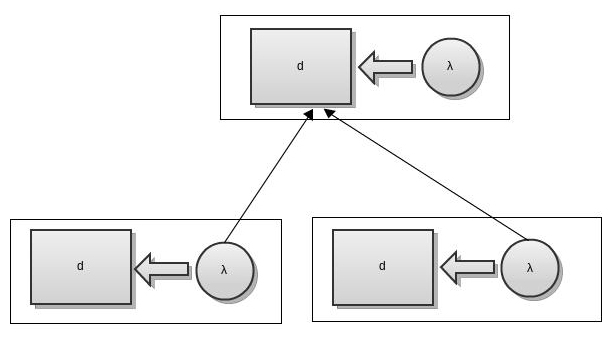
\includegraphics[width=100mm]{./images/label_digest.jpg}
        \caption[]{Labels and Digests}
        \label{fig:labels-and-digests}
        \end{figure}

	The key homomorphic property, which will only be briefly described here, allows every node in the tree to be represented by a sum of representations of all its children.
	Each of those children can be represented as a sum of their children and so on.
	In this way, even the root of the tree can be represented by a sum of representations of the leaves of the tree.
	The representation being alluded to is called a \textit{partial digest} and is calculated for a node, \textit{with respect to} some node in that parent's subtree.
	
	For example, suppose a tree is to represent a set of elements drawn from a universe on integers in $0 \leq x \leq 7$.
	If then we want to represent the root of such a tree in which the set of nodes \{1, 4, 6, 7\} are present, then digest of the root of the tree can be expressed as a sum of partial digests of the root, with respect to the present elements.
	That is $\textit{D}(root, 1)+\textit{D}(root, 4)+\textit{D}(root, 6)+\textit{D}(root, 7)$ where $\textit{D}(root, x)$ is the partial digest of the root with respect to x.
	This type of hash function is what allows the client (verifier) to maintain a correct running digest of all the stream elements seen, regardless of how large the tree is or how many stream elements have been witnessed.
       	
	For the readers knowledge, we describe the hash function, but will not go into detail.  The proof of its security and correctness properties can be found in \cite{sads}.
	The hash function is:
	
	\begin{equation}
		h(x,y)= \textbf{L} x + \textbf{R}y
	\end{equation}
	where $x, y$ are labels of nodes, $\textbf{L}, \textbf{R}$ are matrices performing the role of a public key in the scheme and $h(x,y)$ is a digest.
		
\section{Properties of Digests and Labels}
	
	\begin{enumerate}
		\item Having a label of a node, its digest can be computed (not necessarily the other way around)
		\item Having the labels of the two children nodes, using the hash functions, the digest of the parent could be computed.
	\end{enumerate}
	
	
\section{ Participants }

	\subsection{ Verifier and Prover }
	
		As mentioned previously, the verifier (or client) is a low resource computational device.
		It is expected that the verifier will not have sufficient storage capacity to store every element of a stream witnessed and as such it has no means to correctly answer queries based on the stream elements.
		To accomplish these tasks, the verifier will rely on a more powerful device.
		The verifier will however have the means to storage a digest, a small representation of all the elements it has seen, with the goal being that it will be able to update its local state efficiently enough so as to not disrupt viewing elements of the stream.
		So, the verifier's only operation during the streaming phase will be to update its local state with some representation of each element of the stream.
		This representation will be the partial digest of the root with respect to the witnessed element as previously discussed.
		
		The prover (server) on the other hand must act somewhat as a database.
		Internally, the prover maintains a representation of the stream elements witnessed such that it can answer queries from the verifier.
		That internal representation is the hash tree mentioned earlier which allows for a node to be update without rehashing its children.
		The verifier exploits this property to maintain and update the root digest of the tree without communication with the prover.
		
		\subsection{ Query Proof }
		
		During or after the streaming phase, the verifier may wish to query the prover (server) for the membership, successor, range, frequency etc of a universe element that maybe or may not have been witnessed.
		The prover is expected to provide and answer to the query as well as a proof that can be efficiently verified by the verifier. 
		Figure \ref{fig:proof} in a visual representation of a membership proof for the green node.
		The set of green nodes comprises the \textit{update path} for the green leaf node
		The set of blue nodes are the \textit{siblings} of the nodes on the update path.
		The prover then responds to a membership query with the computed answer as well as the set of sibling pairs which the verifier can then verify.
		
		Verification is done in two parts.
		First, for each sibling pair is hashed to obtain a digest of their parent.
		That calculated digest must be an equivalent representation of the label in the next pair representing this pairs parent.
		Lastly, the digest produced by hashing the last pair of children must be equivalent to the running digest the verifier has been maintaining.
		Shi and Papamanthou \cite{dads} describe the correctness properties in much more detail.
		
		\begin{figure}[h]
		\centering
		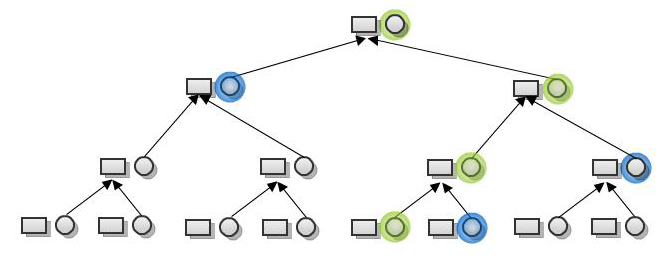
\includegraphics[width=100mm]{./images/8.jpg}
		\caption[]{Prover}
		\label{fig:proof}
		\end{figure}
	

\section{ Implementation }
	
	Implementing the SADS scheme was organized as follows.
	First to be implemented was the data underlying structure used by the prover and mechanisms used by both prover and verifier to support the SADS scheme.
	Then the data structures and mechanism to support the query phase was added.
	Finally, these two parts were packaged such that another project may leverage the SADS scheme as a library primitive and build applications.
	
	Our language of choice for this first stage of the project was Ruby.
	Ruby's main advantage was the ease of rapid prototyping as well as the vast collection of libraries to enhance development and functionality available.
	Specifically, the main component of the SADS scheme is the hash function which require matrix multiplication support.
	Ruby's standard library includes Vector and Matrix arithmetic operations which were sufficient for prototype scale implementations.
	Ruby is also a forward looking choice as we still have the option to create bindings for C and C++ code, should we require more efficient linear algebra libraries.
	
	The implementation in its current state as of this writing consists of two Ruby classes and one Ruby module.
	The classes are, not surprising, Prover and Verifer and the module is named Sads.
	Ruby has a feature called \textit{mixing} in which a module can be "mixed into" a class.
	Mixing in a module has the effect of include all the modules fields and methods into the class definition.
		
	
	
	
	\subsection{Underlying Data Structures}

		A crucial component of the SADS algorithm relies on matrix multiplication, a relatively expensive computational operation.
		When formulating our plan of action for this project, we were recommended a few linear algebra libraries, which will be discussed in a later section.
		While we recognize the importance of fast matrix operations and parallelism for production quality code, we thought that the added complexity, as well as unknowns with respect to implementation details, would be prohibitive.
		Instead, we've decided to use an interpreted language and the simple matrix operations that come with the standard libraries to start.

	
	\subsection{SADS Scheme}

	Once the underlying data structure is complete, the SADS scheme will use it as a primitive.
	Though one of the scheme's strengths is the independence of the prover and verifier during the streaming setting, the two parties will necessarily need to communicate during the query phase.
	Additionally, there may be communication between the two parties to initiate the streaming setting.
	For these reasons, we anticipate creating an application which will require network communication as it will likely be the case that the verifier and prover are not collocated.

	%We have a few frameworks in mind for this task.
	%Two of our options at the moment are EventMachine and Node.js.
	%Node.js is a "platform for building fast, scalable network applications" and has been gaining popularity in the Ruby community. http://nodejs.org/
	%EventMachine is a "fast, simple event-processing library for Ruby programs."http://rubyeventmachine.com/


\section{Looking Forward}

	\subsection{ Benchmarking }
	
	The next stage of development is benchmarking to understand the performance of the implementation and to differentiate constraints resulting from particular design decisions from those arising from the schemes protocol itself.
	We will focus primarily on benchmarking the timing of important operations in the scheme as well as the memory footprint of the implementations largest data structures.
	
	We ran some preliminary calculations to ballpark the size of matrices L and R, the public key of the SADS scheme.
	Recall that L and R are matrices with elements in $Z_q$, that is elements are integers of at most q and q is derived from the security parameter, k and the upper bound on the size of the stream, n.
	So a rough estimate of the size of L and R can be calculated by multiplying the dimensions of the matrices, by the amount of space required for each element.
	Below are two tables of estimations.
	
	\begin{table}[h]
	\centering
	
		\begin{tabular} { c | c | c | c}
		
		k & n & Matrix dim & Footprint\\ \hline
		1000&100000&1000 x 3000&14MB\\
		10000&100000&10000 x 30000&1716MB\\
		100000&100000&100000 x 300000&171661MB\\
		1000000&100000&1000000 x 3000000&20027160MB\\
		10000000&100000&10000000 x 30000000&2288818359MB\\	
		\end{tabular}
	
	\caption{Estimation of public key size.  Constant stream size upper bound , varying security parameter } 
	\label{tab:pub-key_k}
	\end{table}
	
	
	\begin{table}[h]
	\centering
		\begin{tabular}{ c | c | c | c}
		k & n & Matrix dim & Footprint\\ \hline
		500&10&500 x 1500&2MB\\
		500&100&500 x 1500&2MB\\
		500&1000&500 x 1500&2MB\\
		500&10000&500 x 1500&2MB\\
		500&100000&500 x 1500&3MB\\
		500&1000000&500 x 1500&3MB\\
		500&10000000&500 x 1500&4MB\\
		500&100000000&500 x 1500&4MB\\
		
		\end{tabular}
	\caption{ Estimation of public key size.  Constant security parameter, varying stream size upper bound }
	\label{tab:pub-key_n}
	\end{table}
	

	The estimated memory footprint of the public key matrices grows rapidly with an increasing security parameter, but slowly with increasing stream size.
	The reason for this is that the scheme calls for matrices of size $k  \times ( k \times \log q )$.
	The matrix size grows faster than $k^2$ because $q$ also depends on $k$.
	Fortunately, the current proposal is to pick one security parameter which is large enough to provide the appropriate security properties for all instances of the SADS scheme.
	
	Future benchmarking efforts will also measure the memory footprint of the prover over time, and the size of a proof for varying parameter sizes. Additionally, we will benchmark the time required to perform the important updating and proof tasks for each of the prover and verifier. 
	


	\subsection{ Production Quality Libraries }
	
	Through our benchmarking and profiling efforts, we hope to identify and fix the bottlenecks in implementation resulting in faster and higher quality code.
	We recognize that the built-in implementations of certain high cost operations, such as matrix multiplication may end up being the limiting factor, and as such we've identified a few options for future optimization.
	We hesitate to invest time and effort into any of these options too soon as we know that our first-draft implementation necessarily has room for improvement, but we outline those options here.

	\begin{enumerate}
	\item \textbf{SciRuby} : A Ruby library providing efficient implementations of linear algebra operations as well as other science, engineering, and visualization packages. \texttt{http://sciruby.com/}
	\item \textbf{NTL 5.5.2} : A free software written in C++ providing data structures and algorithms for arbitrary length integers, for vectors, matrices and polynomials over the integers and over the finite fields and for arbitrary precision floating point arithmetic. \texttt{http://shoup.net/ntl/}
	\item \textbf{MAGMA V2.18} : The kernel of Magma contains implementations of many of the important concrete classes of structure in five fundamental branches of algebra, namely group theory, ring theory, field theory, module theory and the theory of algebras.
	In addition, certain families of structures from algebraic geometry and finite incidence geometry are included. \texttt{http://magma.maths.usyd.edu.au/}
	\end{enumerate}

	
	%\subsection{Semester Outlook}
		%While the ultimate goal of the project is to produce a proof-of-concept application which utilizes a SADS scheme, it is best to set manage expectations.
		%Our baseline target for this semester is to complete the first two layers described above, that is the underlying data structure and the SADS scheme primitive.
		%Having completed these two components, we can then establish time line during which the proof-of-concept application can be hashed out and developed.
		%We hope to leverage the Ruby and broader open-source community by packaging this application, or just the SADS scheme primitive, into a library for others to use and provide feedback.


%%%%%%%%%%%%%%%%%%%%%%%%%%%%%%%%%%%%%%%%%%%%%%%%%%%%%%%%%%%%%%%%%%%%%%%%

\begin{thebibliography}{9}
	\bibitem{sads} Elaine Shi, Charalampos Papamanthou \emph{Streaming Authenticated Data Structures}, Date Unknown
	\bibitem{evsc} B. Applebaum, Y. Ishai
and E. Kushilevitz \emph{From Secrecy to Soundness:
Efficient Verification via Secure Computation}
	\end{thebibliography}

\end{document}
